\documentclass[tikz,border=10pt]{standalone}
\usetikzlibrary{shapes.geometric, arrows.meta, positioning, fit, backgrounds, calc}
\usepackage{xcolor}

\begin{document}
% We simulate the resizebox effect by just making the distinct parts cleaner, 
% ensuring it scales well. In the main latex file we will wrap this with \resizebox{\linewidth}{!}{...}
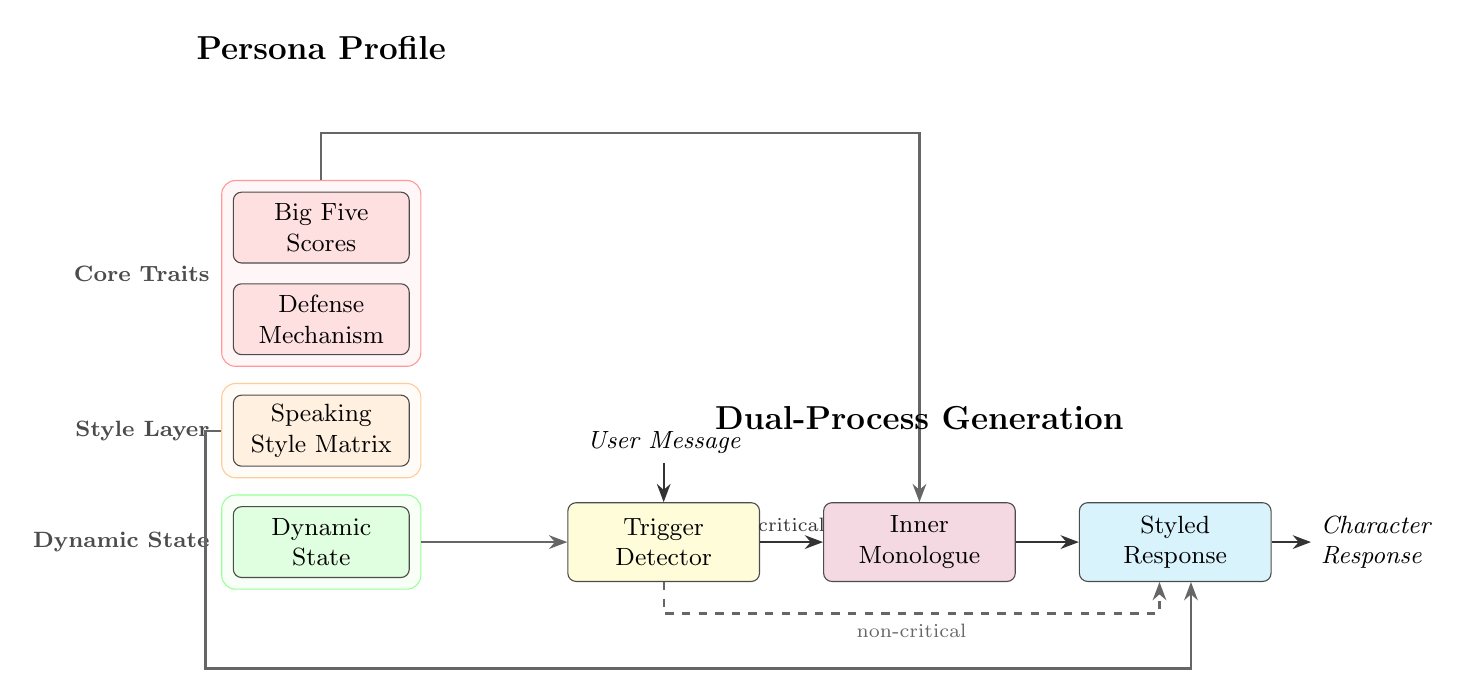
\begin{tikzpicture}[
    node distance=0.4cm and 0.8cm, % Reduced horizontal distance
    box/.style={rectangle, rounded corners=3pt, draw=black!70, text width=2.0cm, minimum height=0.9cm, align=center, font=\small},
    pipelinebox/.style={rectangle, rounded corners=3pt, draw=black!70, text width=2.2cm, minimum height=1.0cm, align=center, font=\small},
    arrow/.style={-{Stealth[scale=1.0]}, thick, black!80},
    dataarrow/.style={-{Stealth[scale=1.0]}, thick, black!60},
    labelstyle/.style={font=\footnotesize\bfseries, black!70, inner sep=2pt}
]

% === Left: Persona Profile Stack ===
\node[box, fill=red!12] (bf) {Big Five\\Scores};
\node[box, fill=red!12, below=0.25cm of bf] (dm) {Defense\\Mechanism};
\node[box, fill=orange!12, below=0.5cm of dm] (style) {Speaking\\Style Matrix};
\node[box, fill=green!12, below=0.5cm of style] (state) {Dynamic\\State};

% Group boxes with tweaked labels
% Group boxes with tweaked labels
% Group boxes with side labels
\begin{scope}[on background layer]
\node[draw=red!40, fill=red!3, rounded corners=5pt, fit=(bf)(dm), inner sep=4pt] (corebox) {};
\node[left=2pt of corebox, labelstyle, anchor=east] {Core Traits};

\node[draw=orange!40, fill=orange!3, rounded corners=5pt, fit=(style), inner sep=4pt] (stylebox) {};
\node[left=2pt of stylebox, labelstyle, anchor=east] {Style Layer};

\node[draw=green!40, fill=green!3, rounded corners=5pt, fit=(state), inner sep=4pt] (statebox) {};
\node[left=2pt of statebox, labelstyle, anchor=east] {Dynamic State};
\end{scope}

% === Right: Dual-Process Pipeline ===
% Move Trigger closer to State horizontally
\node[pipelinebox, fill=yellow!15, right=2.0cm of state] (trigger) {Trigger\\Detector};
\node[pipelinebox, fill=purple!15, right=0.8cm of trigger] (inner) {Inner\\Monologue};
\node[pipelinebox, fill=cyan!15, right=0.8cm of inner] (styled) {Styled\\Response};

% Input/Output labels
\node[above=0.5cm of trigger, font=\itshape\small] (input) {User Message};
\node[right=0.5cm of styled, font=\itshape\small, align=left] (output) {Character\\Response};

% === Pipeline Arrows ===
\draw[arrow] (input) -- (trigger);
\draw[arrow] (trigger) -- node[above, font=\scriptsize, midway] {critical} (inner);
\draw[arrow] (inner) -- (styled);
\draw[arrow] (styled) -- (output);

% === Data Flow Arrows (Routing) ===

% 1. Core Traits -> Inner Monologue (High Road)
% Standard start point now that label is on the side
\draw[dataarrow] (corebox.north) -- ++(0,0.6) -| (inner.north);

% 2. Dynamic State -> Trigger (Direct)
\draw[dataarrow] (statebox.east) -- (trigger.west);

% 3. Speaking Style -> Styled Response (Low Road)
% Route under the statebox to avoid clutter
\draw[dataarrow] (stylebox.west) -- ++(-0.2,0) |- ([yshift=-1.0cm]statebox.south) -| ([xshift=0.2cm]styled.south);

% === Non-Critical Path (Dashed) ===
\draw[arrow, dashed, black!60] (trigger.south) -- ++(0,-0.4) -| node[pos=0.25, below, font=\scriptsize] {non-critical} ([xshift=-0.2cm]styled.south);

% === Section Labels ===
% Positioned relative to the overall groups
\node[above=1.4cm of corebox, font=\large\bfseries] {Persona Profile};
\node[above=0.8cm of inner, font=\large\bfseries] {Dual-Process Generation};

\end{tikzpicture}
\end{document}
